\سؤال{قبل از بهبود عمل‌کرد}

پس از اجرای برنامه و تابع \lr{main}، با استفاده از ابزار \lr{Yourkit} وضعیت برنامه و منابع استفاده شده به شکل زیر است:

\begin{figure}[!hbpt]
	\centering
	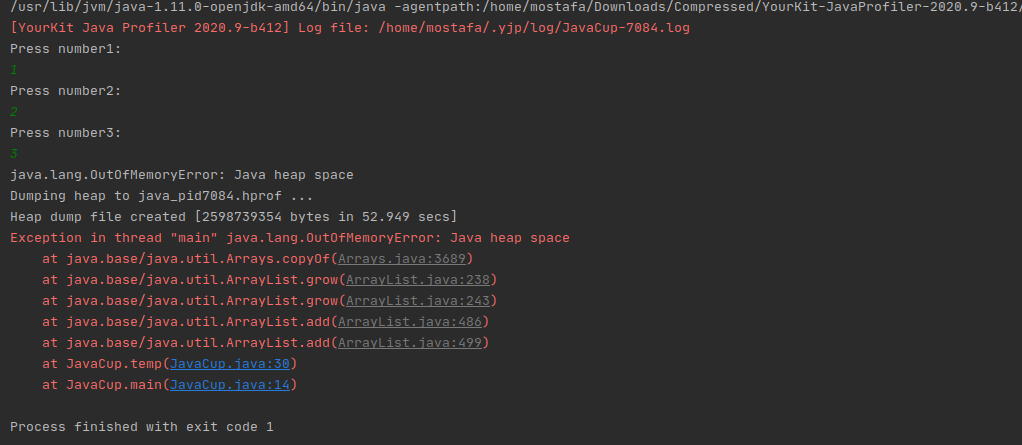
\includegraphics[scale=0.35]{./img/before/3.png}
	\caption{برنامه بعد از اجرا قبل از بهبود عمل‌کرد}
\end{figure}


\begin{figure}[!hbpt]
	\centering
	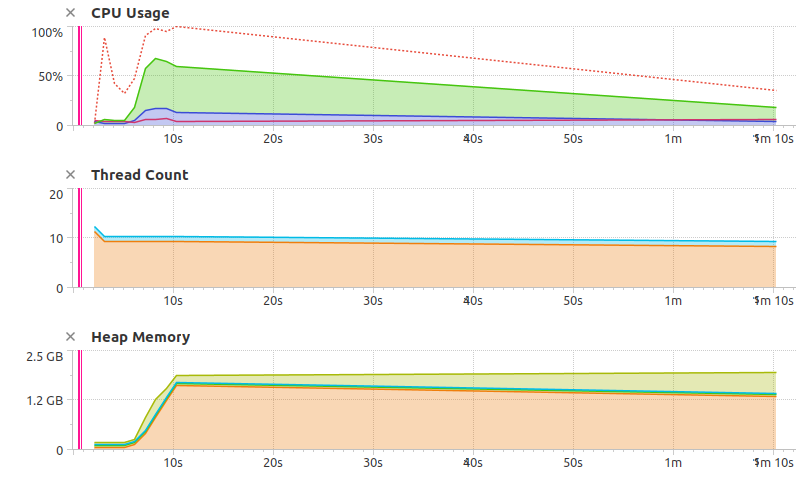
\includegraphics[scale=0.5]{./img/before/1.png}
	\caption{نمودار منابع استفاده شده قبل از بهبود عمل‌کرد}
\end{figure}


و همان‌طور که مشاهده و برداشت می‌شود، تابع \lr{temp} بیش‌ترین مصرف منابع را دارد و حافظه و پردازنده‌ را به شدت درگیر می‌کند.

\begin{figure}[!hbpt]
	\centering
	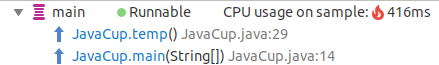
\includegraphics[scale=0.5]{./img/before/2.png}
	\caption{توابع استفاده شده قبل از بهبود عمل‌کرد}
\end{figure}


\begin{figure}[!hbpt]
	\centering
	
\includegraphics[scale=0.5]{./img/before/4.png}
	\caption{میزان \lr{heap} استفاده شده قبل از بهبود عمل‌کرد}
\end{figure}




\begin{figure}[!hbpt]
	\centering
	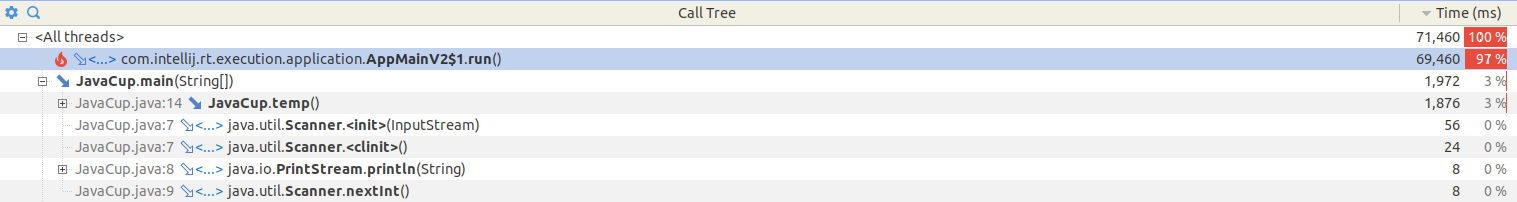
\includegraphics[width=\linewidth]{./img/before/5.png}
	\caption{زمان اجرای توابع قبل از بهبود عمل‌کرد}
\end{figure}

\newpage

 \سؤال{بعد از بهبود عمل‌کرد}
 
برای بهبود عمل‌کرد، باید پیاده‌سازی آن را با قطعه کد زیر جای‌گزین کنیم:

\begin{Verbatim}[tabsize=4]
public static void temp() {
	int[] a = new int[200000000];
	int counter = 0;
	for (int i = 0; i < 10000; i++)
	{
		for (int j = 0; j < 20000; j++) {
		a[counter] = i + j;
		counter += 1;
		}
	}
}
\end{Verbatim}

دلیل پر شدن \lr{heap}، استفاده از \lr{ArrayList} است. زیرا این داده‌ساختار فضای پویا می‌گیرد و هر بار که فضای آن پر می‌شود، مقدار فضای اختصاص‌داده را دو برابر می‌کند. به همین علت باعث مصرف بالای منابع می‌شود.
اما در این قسمت چون تعداد خانه‌هایی که لازم است اختصاص دهیم مشخص است، می‌توانیم در ابتدا آن را مشخص کنیم و جلوی مشکل پیش‌آمده را بگیریم.

در نهایت پس از اعمال تغییرات، اگر بار دیگر با استفاده از ابزار \lr{Yourkit} برنامه را اجرا کنیم، وضعیت استفاده از منابع به شکل زیر می‌شود.

\begin{figure}[!hbpt]
	\centering
	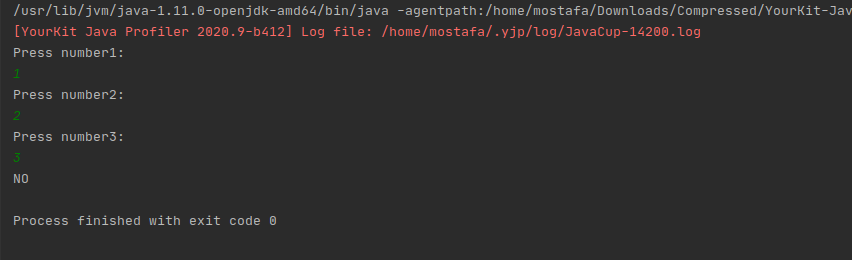
\includegraphics[scale=0.4]{./img/after/2.png}
	\caption{نتیجه اجرای برنامه بعد از بهبود عمل‌کرد}
\end{figure}

\begin{figure}[!hbpt]
	\centering
	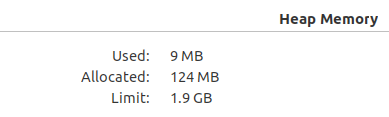
\includegraphics[scale=0.5]{./img/after/3.png}
	\caption{میزان \lr{heap} استفاده شده بعد از بهبود عمل‌کرد}
\end{figure}

\begin{figure}[!hbpt]
	\centering
	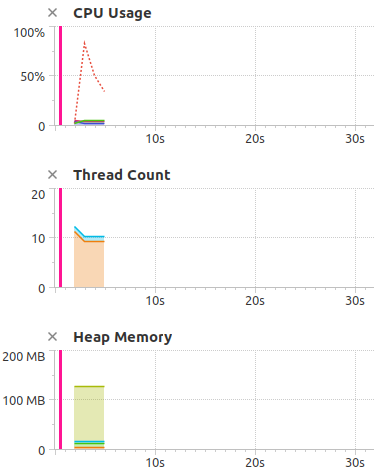
\includegraphics[scale=0.4]{./img/after/1.png}
	\caption{نمودار منابع استفاده شده بعد از بهبود عمل‌کرد}
\end{figure}

\begin{figure}[!hbpt]
	\centering
	
\includegraphics[width=\linewidth]{./img/after/4.png}
	\caption{زمان اجرای توابع بعد از بهبود عمل‌کرد}
\end{figure}